\chapter{Phân tích và thiết kế hệ thống}
\label{chap:phantich}

\sloppy

Chương này trình bày yêu cầu, mô hình ca sử dụng, kiến trúc cùng các quyết định thiết kế chính, và thiết kế luồng xử lý, lớp, cơ sở dữ liệu, giao diện.

\section{Phân tích yêu cầu}
\label{sec:yeucau}

\subsection{Các tác nhân}

Hệ thống có ba tác nhân. \textbf{Người dùng} là người dân hoặc người làm công tác pháp lý cần biết một hành vi bị xử phạt thế nào; câu hỏi thường dùng ngôn ngữ đời thường, có thể không dấu hoặc viết tắt. \textbf{Người phát triển} nạp văn bản mới, chạy các bộ đánh giá và theo dõi chất lượng tìm kiếm. \textbf{Agent} là mô hình ngôn ngữ lớn chạy không tương tác, chỉ được gọi bốn công cụ tra cứu chỉ đọc qua MCP để tìm điều khoản và soạn câu trả lời.

\subsection{Yêu cầu chức năng}

Các yêu cầu chức năng của hệ thống được tổng hợp trong Bảng~\ref{tab:yc-chucnang}.

\begin{table}[H]
\centering
\caption{Yêu cầu chức năng của hệ thống}
\label{tab:yc-chucnang}
\footnotesize
\begin{tabularx}{\textwidth}{@{}l X l@{}}
\toprule
\textbf{Mã} & \textbf{Yêu cầu} & \textbf{Tác nhân} \\
\midrule
FR01 & Trả lời câu hỏi viết bằng tiếng Việt tự nhiên, kể cả không dấu hoặc viết tắt; câu trả lời ngắn gọn, mỗi khẳng định có trích dẫn trỏ tới điều khoản nguồn & Người dùng \\
FR02 & Hiển thị nguyên văn điều khoản được trích, kèm số hiệu văn bản, địa chỉ Điều--Khoản--Điểm và ngày hiệu lực & Người dùng \\
FR03 & Tra cứu điều khoản theo một tình huống và trả về nguyên văn, không qua tóm tắt & Người dùng \\
FR04 & Lọc kết quả theo ngày xảy ra vi phạm, chỉ giữ quy định còn hiệu lực vào ngày đó, và theo danh sách văn bản & Người dùng \\
FR05 & Chế độ ``Tra cứu kỹ hơn'': agent tự diễn đạt lại truy vấn, tra cứu qua nhiều bước rồi lựa chọn điều khoản & Người dùng, Agent \\
FR06 & Gắn ghi chú khi một điều khoản đã bị văn bản khác sửa đổi, bổ sung hoặc bãi bỏ và quy định sửa đổi đã có hiệu lực & Người dùng \\
FR07 & Kiểm tra câu trả lời bám nguồn: số hiệu Điều và số tiền trong câu trả lời phải xuất hiện trong các điều khoản được trích; nếu không, yêu cầu agent trả lời lại một lần & Hệ thống \\
FR08 & Chuyển ngôn ngữ giao diện Việt/Anh và chế độ màu sáng, tối hoặc tự động & Người dùng \\
FR09 & Nạp văn bản Word: chuyển thành văn bản chuẩn, phân tích cấu trúc, tạo đoạn, liên kết trích dẫn và tính vector & Người phát triển \\
FR10 & Cung cấp bốn công cụ tra cứu chỉ đọc qua máy chủ MCP & Agent \\
FR11 & Xem, chỉnh sửa và chạy bộ đánh giá tìm kiếm trên giao diện; chạy bộ đánh giá câu trả lời bằng dòng lệnh & Người phát triển \\
FR12 & Xuất và nhập toàn bộ cơ sở dữ liệu dưới dạng bản chụp (snapshot) để tái lập kết quả đo & Người phát triển \\
\bottomrule
\end{tabularx}
\end{table}

\subsection{Yêu cầu phi chức năng}

Để có thể kiểm chứng, mỗi yêu cầu phi chức năng được gắn với một chỉ tiêu định lượng. Bảng~\ref{tab:yc-phichucnang} nêu chỉ tiêu do nhóm đặt ra và kết quả đo thực tế trên kho 14 văn bản gồm 6.775 đoạn; kết quả tìm kiếm được đo trên bộ 715 câu (592 câu dev, 123 câu holdout), còn kết quả câu trả lời được đo trên bộ 81 câu, trong đó 71 câu thuộc phạm vi kho văn bản.

\begin{table}[H]
\centering
\caption{Yêu cầu phi chức năng, chỉ tiêu và kết quả đo}
\label{tab:yc-phichucnang}
\footnotesize
\begin{tabularx}{\textwidth}{@{}l X l l@{}}
\toprule
\textbf{Mã} & \textbf{Yêu cầu} & \textbf{Chỉ tiêu} & \textbf{Kết quả đo} \\
\midrule
NFR01 & Độ phủ tìm kiếm: điều khoản đáp án nằm trong kết quả của lời gọi tìm kiếm đầu tiên & $\geq 90\%$ & 93,4\% dev; 97,6\% holdout \\
NFR02 & Độ chính xác câu trả lời: đúng Điều, đủ mức tiền, đủ dữ kiện và bám nguồn & $\geq 90\%$ & 97,2\% (69/71) \\
NFR03 & Số liệu trong câu trả lời bám nguồn & $\geq 95\%$ & 98,8\% \\
NFR04 & Không từ chối nhầm câu hỏi trong phạm vi & 0\% & 0\% \\
NFR05 & Độ trễ tra cứu một lần, gồm mã hoá câu hỏi trên CPU và truy vấn cơ sở dữ liệu & p95 $\leq 1$ s & p50 501 ms; p95 690 ms \\
NFR06 & Độ trễ trả lời ở chế độ agent & trung vị $\leq 60$ s & 36 s; chậm nhất 105 s \\
NFR07 & Chi phí gọi mô hình cho mỗi câu hỏi ở chế độ agent & $\leq 0{,}20$ USD & 0,159 USD \\
NFR08 & Mô hình embedding chạy được trên GPU 4 GB & 4 GB & Qwen3-Embedding-0.6B, 512 chiều \\
NFR09 & An toàn: agent chỉ được gọi công cụ chỉ đọc & 4 công cụ & 4 công cụ, tối đa 10 lượt, 300 s \\
NFR10 & Tổng quát hoá: nạp văn bản mới không cần sửa mã nguồn & 0 dòng mã & 14 văn bản dùng chung một bộ phân tích \\
NFR11 & Tái lập: cùng một bản chụp dữ liệu cho cùng kết quả đo & tất định & Lược đồ theo phiên bản, bản chụp JSONL \\
NFR12 & Khả dụng: song ngữ, ba chế độ màu, dùng được trên điện thoại & có & có \\
\bottomrule
\end{tabularx}
\end{table}

Hai chỉ tiêu độ trễ chênh nhau một bậc độ lớn là có chủ đích: tra cứu một lần phải đủ nhanh để tương tác trực tiếp, còn chế độ agent đổi thời gian và chi phí lấy độ chính xác.

\section{Mô hình ca sử dụng}
\label{sec:usecase}

Biểu đồ ca sử dụng tổng quát được trình bày ở Hình~\ref{fig:usecase}. Ca ``Lọc theo ngày vi phạm và văn bản'' mở rộng ca tra cứu điều luật; ca ``Tra cứu kỹ hơn bằng agent'' mở rộng cả ca hỏi đáp lẫn ca tra cứu, đồng thời bao hàm ca ``Gọi công cụ tra cứu MCP'' của tác nhân Agent.

\begin{figure}[H]
\centering
\resizebox{0.82\textwidth}{!}{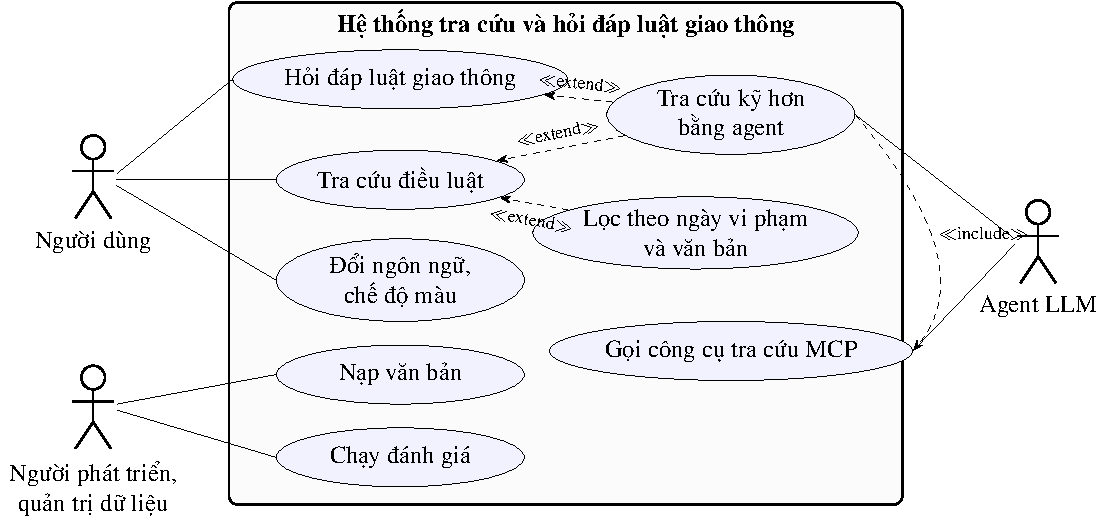
\includegraphics{graphics/fig_ch3_1.pdf}}
\caption{Biểu đồ ca sử dụng tổng quát}
\label{fig:usecase}
\end{figure}

Bảng~\ref{tab:uc-hoidap} và Bảng~\ref{tab:uc-tracuu} đặc tả hai ca sử dụng chính của người dùng; ca nạp văn bản được mô tả bằng biểu đồ hoạt động ở Mục~\ref{sec:luongxuly}.

\begin{table}[H]
\centering
\caption{Đặc tả ca sử dụng UC01: Hỏi đáp luật giao thông}
\label{tab:uc-hoidap}
\footnotesize
\begin{tabularx}{\textwidth}{@{}p{2.8cm} X@{}}
\toprule
\textbf{Tên ca sử dụng} & Hỏi đáp luật giao thông \\
\textbf{Tác nhân} & Người dùng (chính), Agent (phụ) \\
\textbf{Tiền điều kiện} & Cơ sở dữ liệu đã nạp kho văn bản; API web đang hoạt động; với chế độ agent, chương trình dòng lệnh gọi mô hình đã được cài đặt trên máy chủ \\
\textbf{Luồng chính} & 1. Người dùng nhập câu hỏi ở thẻ ``Hỏi đáp'' và giữ lựa chọn ``Tra cứu kỹ hơn''. \newline
2. Giao diện gửi yêu cầu trả lời ở chế độ agent tới API. \newline
3. Hệ thống khởi chạy agent; agent gọi các công cụ tra cứu, chọn nguồn và soạn câu trả lời có đánh số trích dẫn. \newline
4. Hệ thống đọc lại các điều khoản nguồn từ cơ sở dữ liệu, gắn ghi chú sửa đổi, đánh số lại trích dẫn và kiểm tra tính bám nguồn. \newline
5. Giao diện hiển thị câu trả lời, danh sách điều khoản nguồn và ghi chú sửa đổi. \\
\textbf{Luồng rẽ nhánh} & 3a. Người dùng bỏ chọn ``Tra cứu kỹ hơn'': hệ thống tìm kiếm một lần rồi gửi mặc định năm điều khoản cho mô hình soạn câu trả lời. \newline
4a. Kiểm tra bám nguồn không đạt: agent được chạy lại một lần kèm phản hồi; hệ thống giữ phương án có ít số liệu thiếu căn cứ hơn. \newline
4b. Ở chế độ tìm kiếm một lần, nếu không kết quả nào chứa cụm từ của câu hỏi, hệ thống thông báo không tìm thấy căn cứ mà không gọi mô hình. \\
\textbf{Ngoại lệ} & Không kết nối được máy chủ MCP, agent vượt quá 300 giây hoặc nhà cung cấp mô hình báo lỗi: API trả mã lỗi kèm lý do và không hiển thị câu trả lời. \\
\textbf{Hậu điều kiện} & Mọi điều khoản hiển thị đều được đọc từ cơ sở dữ liệu, không phải nội dung do agent tự chép lại. \\
\bottomrule
\end{tabularx}
\end{table}

\begin{table}[H]
\centering
\caption{Đặc tả ca sử dụng UC02: Tra cứu điều luật có bộ lọc}
\label{tab:uc-tracuu}
\footnotesize
\begin{tabularx}{\textwidth}{@{}p{2.8cm} X@{}}
\toprule
\textbf{Tên ca sử dụng} & Tra cứu điều luật (mở rộng: lọc theo ngày vi phạm và văn bản) \\
\textbf{Tác nhân} & Người dùng \\
\textbf{Tiền điều kiện} & Cơ sở dữ liệu đã nạp kho văn bản \\
\textbf{Luồng chính} & 1. Người dùng mô tả tình huống ở thẻ ``Tra cứu điều luật''. \newline
2. Người dùng mở bộ lọc, chọn ngày xảy ra vi phạm và một hoặc nhiều văn bản. \newline
3. Giao diện gửi yêu cầu tìm kiếm kèm ngày vi phạm và danh sách văn bản tới API. \newline
4. Hệ thống tìm kiếm lai theo vector và BM25, chỉ giữ các đoạn còn hiệu lực vào ngày vi phạm và thuộc các văn bản đã chọn, đồng thời gắn ghi chú sửa đổi. \newline
5. Giao diện hiển thị nguyên văn từng điều khoản, ngày hiệu lực và nút xem ngữ cảnh. \\
\textbf{Luồng rẽ nhánh} & 2a. Người dùng không chọn ngày: ngày vi phạm mặc định là ngày hiện tại theo giờ Việt Nam. \newline
3a. Người dùng chọn ``Tra cứu kỹ hơn'': agent lựa chọn tối đa năm điều khoản thay cho kết quả tìm kiếm thô. \newline
5a. Độ tin cậy thấp: giao diện hiển thị cảnh báo phía trên kết quả. \\
\textbf{Hậu điều kiện} & Kết quả là nguyên văn điều luật, không qua tóm tắt. \\
\bottomrule
\end{tabularx}
\end{table}

\section{Kiến trúc tổng thể}
\label{sec:kientruc}

\subsection{Kiến trúc phân tầng}

Hệ thống gồm bốn tầng (Hình~\ref{fig:kientruc}). Tầng nạp văn bản chuyển tài liệu gốc thành cây phân cấp, các đoạn và các cạnh trích dẫn. Tầng lưu trữ dùng PostgreSQL với \texttt{pgvector}, \texttt{ltree} và \texttt{unaccent}, để văn bản, vector, chỉ mục từ khoá và đồ thị trích dẫn cùng nằm trong một cơ sở dữ liệu. Tầng tra cứu và agent đóng gói các thao tác tìm kiếm, duyệt cây, duyệt đồ thị và ghi chú sửa đổi thành công cụ MCP cho agent. Tầng trên cùng gồm API web, giao diện và công cụ đánh giá.

\begin{figure}[H]
\centering
\resizebox{0.82\textwidth}{!}{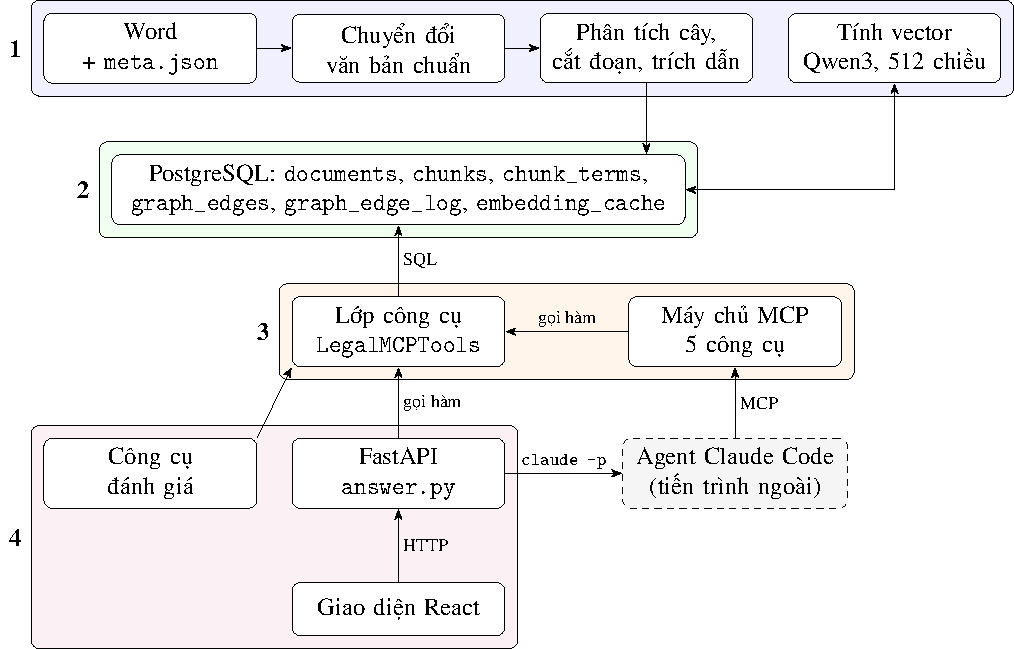
\includegraphics{graphics/fig_ch3_2.pdf}}
\caption{Kiến trúc bốn tầng: (1) nạp văn bản, (2) lưu trữ, (3) tra cứu và agent, (4) API, giao diện và đánh giá}
\label{fig:kientruc}
\end{figure}

\subsection{Các quyết định thiết kế chính}

Kiến trúc dựa trên năm quyết định thiết kế, mỗi quyết định giải quyết một đặc thù của văn bản quy phạm pháp luật tiếng Việt.

\begin{enumerate}
    \item \textbf{Phân tích cấu trúc tất định.} Văn bản được dựng thành cây Điều--Khoản--Điểm theo quy ước đánh số thay vì cắt theo độ dài cố định; hệ thống kiểm tra mỗi dòng có nội dung thuộc đúng một đoạn để lỗi phân tích không làm mất nội dung âm thầm.
    \item \textbf{Lưu nguyên văn và văn bản kèm ngữ cảnh.} Vì mức phạt nằm ở câu dẫn của Khoản còn hành vi nằm ở Điểm, mỗi đoạn được lưu thêm một phiên bản ghép tên văn bản và các câu dẫn cấp trên để tính vector và lập chỉ mục.
    \item \textbf{Tìm kiếm lai.} Nhánh vector nắm bắt ngữ nghĩa; nhánh BM25 trên âm tiết không dấu xử lý tốt câu không dấu và số hiệu; hai nhánh được hợp nhất bằng RRF, kèm tìm kiếm theo cụm từ ở tầng công cụ.
    \item \textbf{Đồ thị trích dẫn và ghi chú sửa đổi đọc từ văn bản.} Mỗi cạnh trích dẫn phải kèm cụm từ có nguyên văn trong điều khoản nguồn; ghi chú sửa đổi được suy ra từ chính các câu lệnh sửa đổi.
    \item \textbf{Kiểm tra bám nguồn.} Agent chỉ trả về câu trả lời và danh sách đường dẫn; hệ thống tự đọc nguyên văn từ cơ sở dữ liệu để hiển thị và đối chiếu số Điều, số tiền trong câu trả lời với nguồn.
\end{enumerate}

\section{Thiết kế luồng xử lý}
\label{sec:luongxuly}

\subsection{Luồng nạp văn bản}

Luồng nạp văn bản (Hình~\ref{fig:activity-ingest}) gồm ba bước độc lập. Bước chuyển đổi đọc tệp Word đúng như cách Word hiển thị rồi làm sạch thành văn bản chuẩn theo dòng; số dòng là hệ toạ độ chung của toàn hệ thống. Bước nạp phân tích cây, tạo đoạn, kiểm tra độ phủ theo dòng, liên kết trích dẫn và ghi toàn bộ kết quả trong một giao dịch. Bước tính vector chạy ngoài giao dịch để quá trình tính trên GPU không giữ khoá cơ sở dữ liệu.

\begin{figure}[H]
\centering
\resizebox{0.85\textwidth}{!}{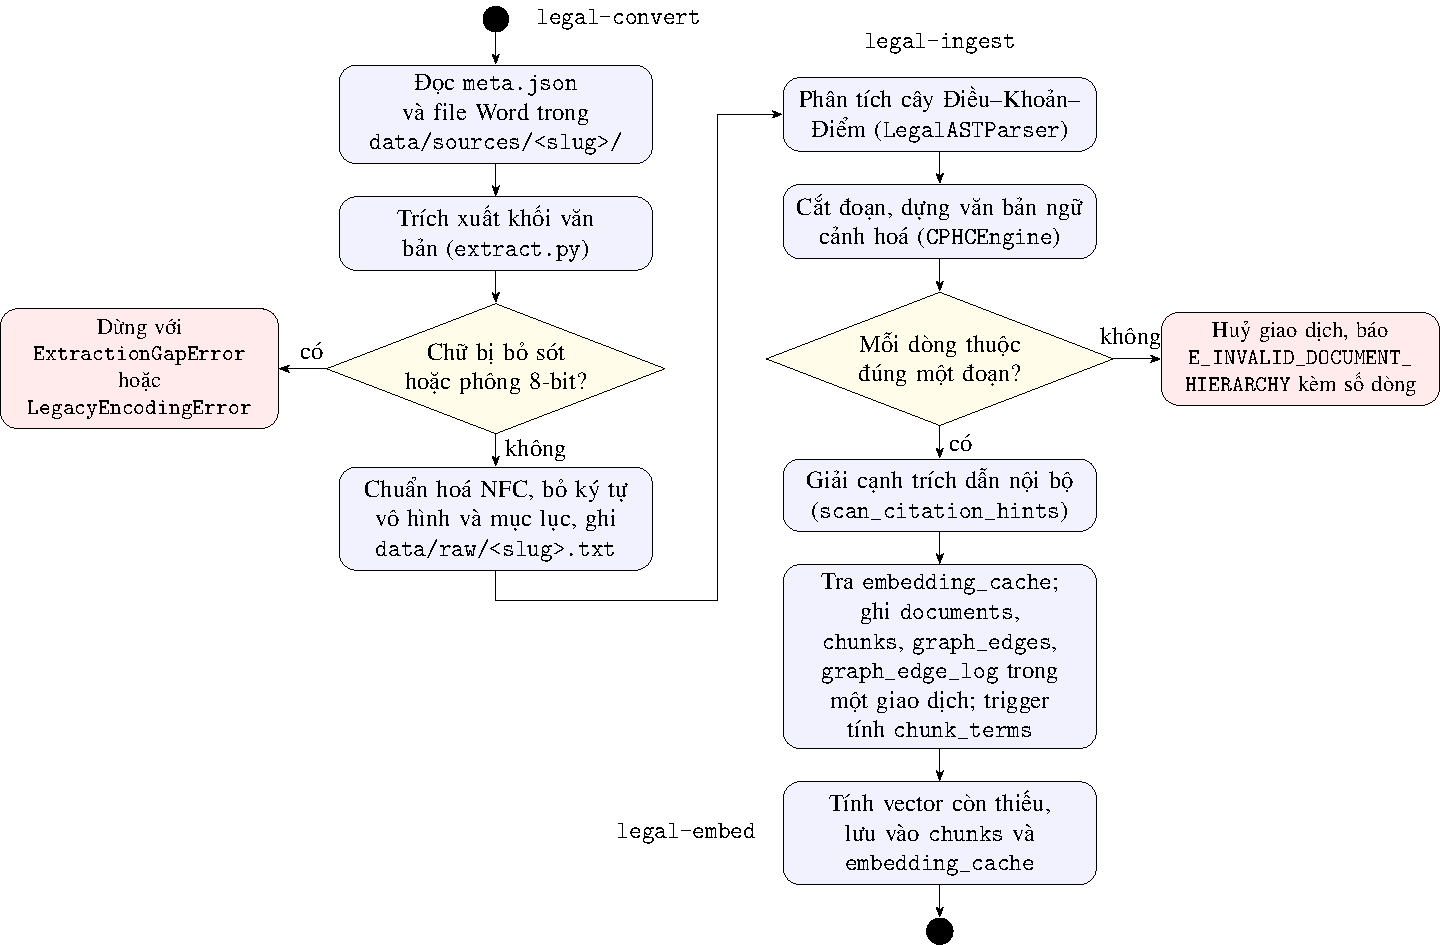
\includegraphics{graphics/fig_ch3_3.pdf}}
\caption{Biểu đồ hoạt động của luồng nạp văn bản}
\label{fig:activity-ingest}
\end{figure}

\subsection{Luồng trả lời ở chế độ agent}

Hình~\ref{fig:sequence-agent} mô tả trình tự xử lý một câu hỏi ở chế độ agent. API khởi chạy agent trong một thư mục tạm, chỉ với máy chủ MCP của hệ thống và bốn công cụ chỉ đọc. Agent tra cứu qua nhiều lượt rồi trả về câu trả lời cùng danh sách nguồn. Hệ thống đọc lại nguyên văn các nguồn từ cơ sở dữ liệu, gắn ghi chú sửa đổi, đánh số lại trích dẫn và kiểm tra bám nguồn; nếu không đạt, agent được chạy lại một lần kèm danh sách số liệu thiếu căn cứ.

\begin{figure}[H]
\centering
\resizebox{0.86\textwidth}{!}{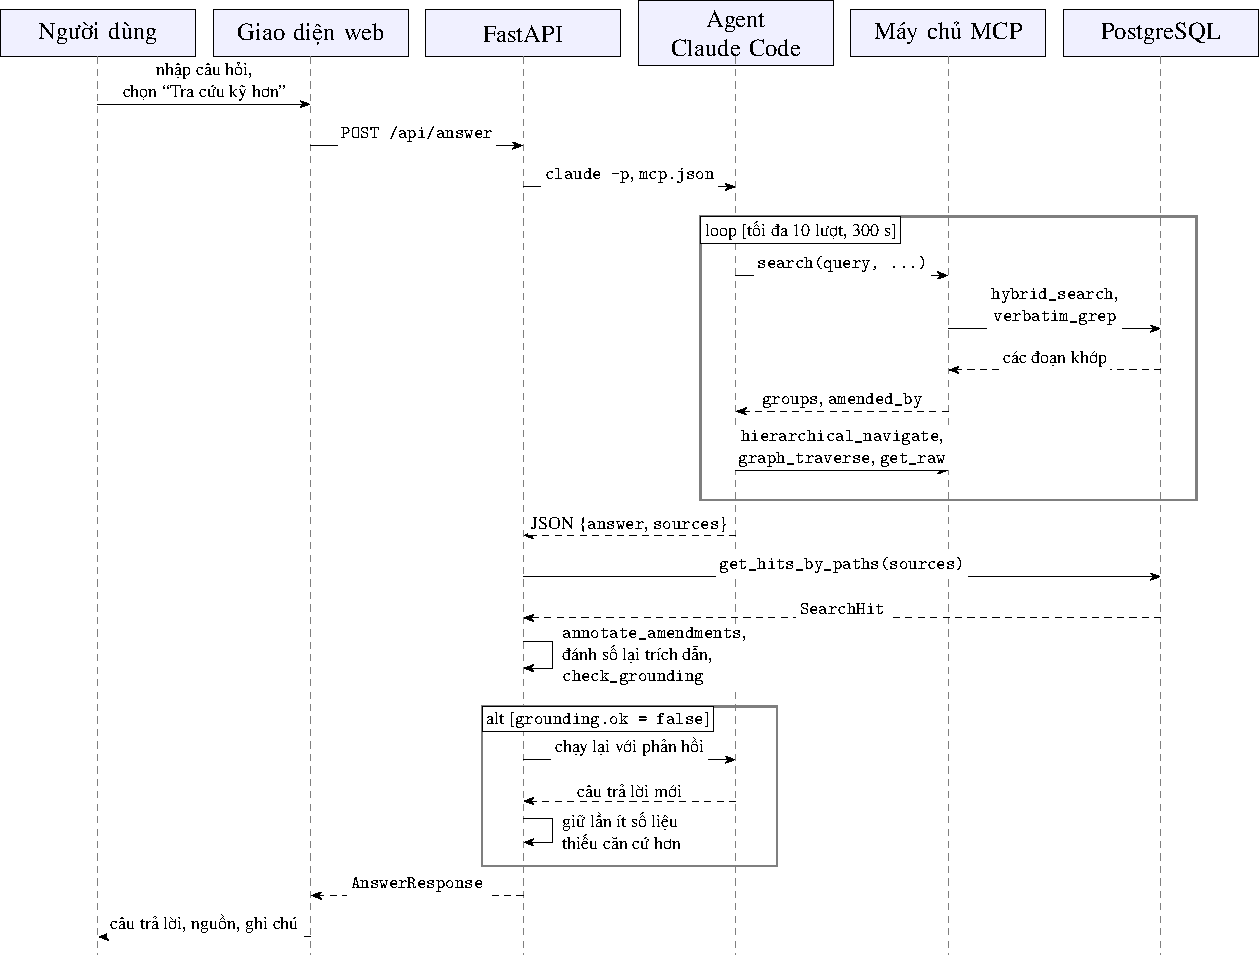
\includegraphics{graphics/fig_ch3_4.pdf}}
\caption{Biểu đồ tuần tự trả lời một câu hỏi ở chế độ agent}
\label{fig:sequence-agent}
\end{figure}

Ở chế độ tìm kiếm một lần, hệ thống bỏ qua vòng lặp gọi công cụ, tìm kiếm trực tiếp rồi gửi các điều khoản tìm được cho mô hình soạn câu trả lời trong một lượt; nếu không có kết quả nào khớp từ khoá của câu hỏi, hệ thống từ chối mà không gọi mô hình.

\section{Thiết kế lớp}
\label{sec:thietkelop}

Hình~\ref{fig:class} trình bày biểu đồ lớp của các module chính. Lớp \texttt{LegalMCPTools} là mặt tiền (facade) gom nhóm công cụ tra cứu chỉ đọc và nhóm công cụ bảo trì đồ thị, được cả máy chủ MCP lẫn API web dùng chung. Mọi kết quả tìm kiếm, duyệt cây và duyệt đồ thị đều được biểu diễn bằng cùng một kiểu \texttt{SearchHit}, có thể kèm nhiều ghi chú sửa đổi.

\begin{figure}[H]
\centering
\resizebox{0.85\textwidth}{!}{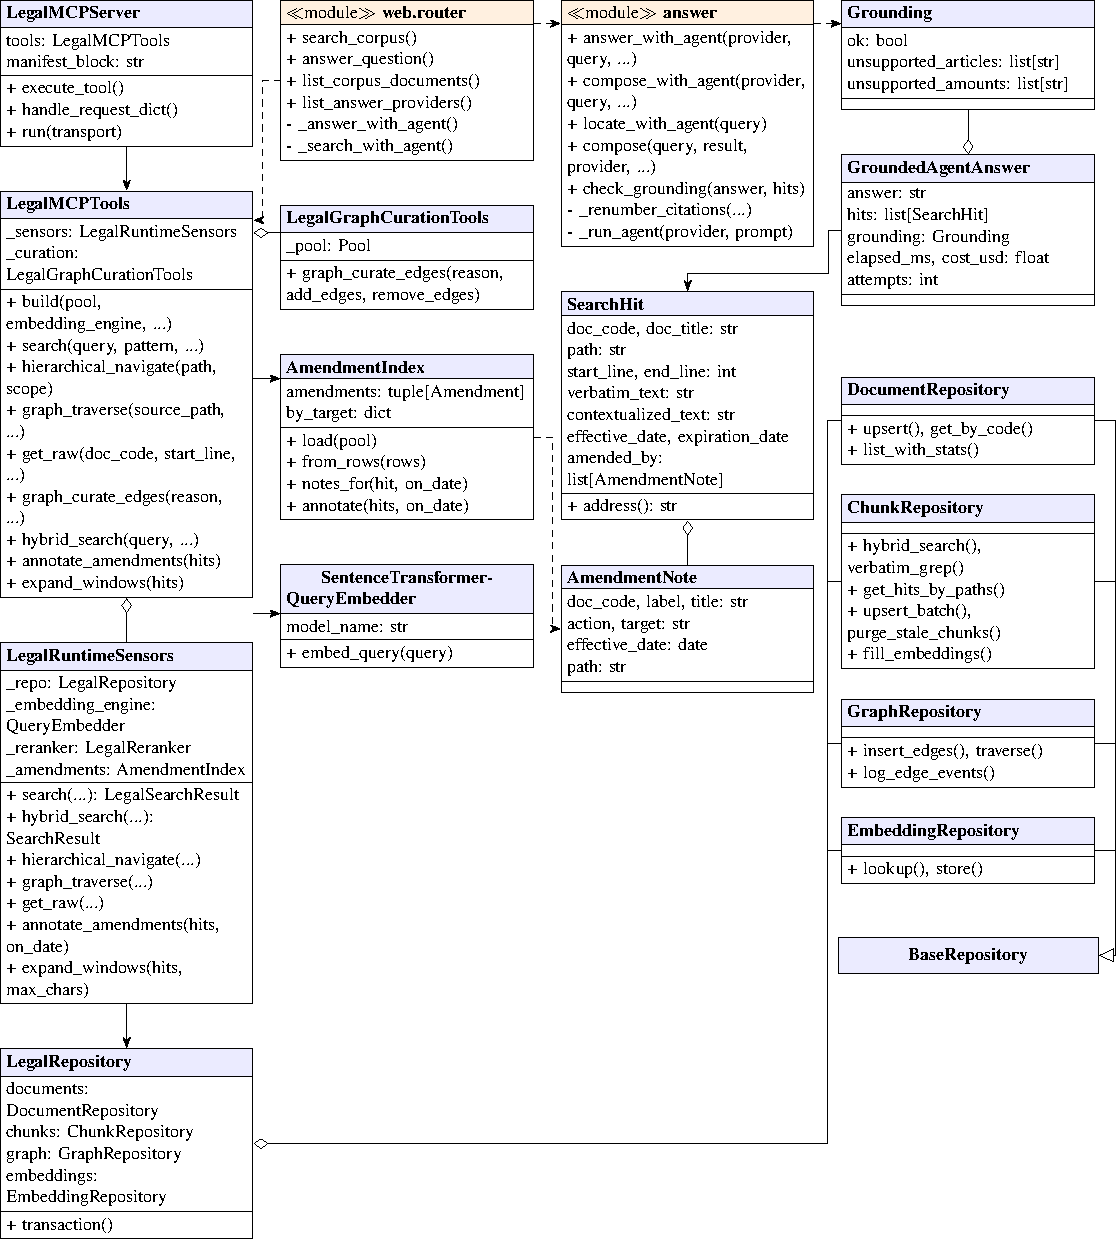
\includegraphics{graphics/fig_ch3_5.pdf}}
\caption{Biểu đồ lớp của các module chính}
\label{fig:class}
\end{figure}

\section{Thiết kế cơ sở dữ liệu}
\label{sec:csdl}

\subsection{Mô hình thực thể liên kết}

Lược đồ được xây dựng qua một chuỗi migration áp dụng theo thứ tự; Hình~\ref{fig:erd} mô tả trạng thái cuối cùng.

\begin{figure}[H]
\centering
\resizebox{\textwidth}{!}{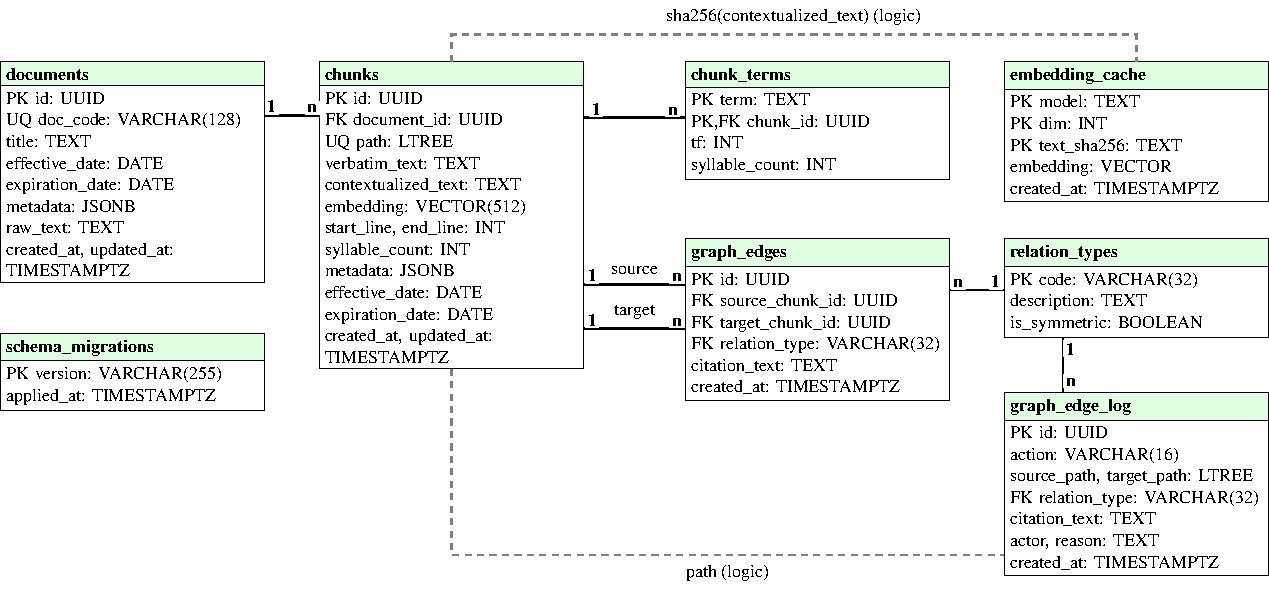
\includegraphics{graphics/fig_ch3_6.pdf}}
\caption{Mô hình thực thể liên kết của cơ sở dữ liệu (nét liền: khoá ngoại; nét đứt: liên kết logic)}
\label{fig:erd}
\end{figure}

Thiết kế có hai điểm đáng chú ý. Thứ nhất, mỗi đoạn được định danh bằng một đường dẫn phân cấp kiểu \texttt{ltree}; chẳng hạn, đường dẫn kết thúc bằng \texttt{a\_6.c\_9.p\_b} ứng với Điểm b Khoản 9 Điều 6, nhờ đó có thể lọc cả một nhánh cây cùng điều kiện hiệu lực ngay trong một câu truy vấn SQL. Thứ hai, bộ đệm vector được khoá theo mô hình, số chiều và mã băm của văn bản, nên vector được dùng lại khi nạp lại văn bản mà nội dung không đổi.

\subsection{Đặc tả các bảng}

Bảng~\ref{tab:db-chunks} đặc tả bảng chính \texttt{chunks}, còn Bảng~\ref{tab:db-khac} tóm tắt các bảng còn lại. Cột ``Ràng buộc'' sử dụng các ký hiệu PK (khoá chính), FK (khoá ngoại), UQ (duy nhất) và NN (không rỗng).

\begin{table}[H]
\centering
\caption{Bảng \texttt{chunks}: đơn vị lưu trữ và tìm kiếm}
\label{tab:db-chunks}
\footnotesize
\setlength{\tabcolsep}{3pt}
\begin{tabularx}{\textwidth}{@{}l l l X@{}}
\toprule
\textbf{Cột} & \textbf{Kiểu} & \textbf{Ràng buộc} & \textbf{Ý nghĩa} \\
\midrule
\texttt{id} & UUID & PK & Định danh đoạn \\
\texttt{document\_id} & UUID & FK, NN & Văn bản chứa đoạn (xoá theo văn bản) \\
\texttt{path} & LTREE & UQ, NN & Đường dẫn phân cấp Chương--Điều--Khoản--Điểm \\
\texttt{verbatim\_text} & TEXT & NN & Nguyên văn các dòng thuộc đoạn \\
\texttt{contextualized\_text} & TEXT & NN & Văn bản đã ghép tên văn bản, các cấp cha và câu dẫn; dùng để tính vector và lập chỉ mục BM25 \\
\texttt{embedding} & VECTOR(512) & & Vector Qwen3-Embedding-0.6B, chỉ mục HNSW theo cosine \\
\texttt{start\_line}, \texttt{end\_line} & INT & NN, CHECK & Phạm vi dòng trong văn bản chuẩn \\
\texttt{syllable\_count} & INT & NN & Số âm tiết, tức độ dài $|d|$ trong BM25; được trigger cập nhật \\
\texttt{metadata} & JSONB & NN & Loại nút, nhãn và tên Chương, Mục, Điều \\
\texttt{effective\_date} & DATE & NN & Ngày có hiệu lực \\
\texttt{expiration\_date} & DATE & CHECK & Ngày hết hiệu lực (rỗng nếu còn hiệu lực) \\
\bottomrule
\end{tabularx}
\end{table}

\begin{table}[H]
\centering
\caption{Các bảng khác của cơ sở dữ liệu}
\label{tab:db-khac}
\footnotesize
\begin{tabularx}{\textwidth}{@{}>{\raggedright\arraybackslash}p{3.4cm} >{\raggedright\arraybackslash}p{2.8cm} X@{}}
\toprule
\textbf{Bảng} & \textbf{Khoá} & \textbf{Nội dung chính} \\
\midrule
\texttt{documents} & PK \texttt{id}, UQ \texttt{doc\_code} & Số hiệu, tên văn bản, ngày hiệu lực và hết hiệu lực, siêu dữ liệu về quan hệ sửa đổi, toàn văn văn bản chuẩn \\
\texttt{chunk\_terms} & PK (\texttt{term}, \texttt{chunk\_id}) & Chỉ mục ngược cho BM25 do trigger duy trì: âm tiết hoặc cặp âm tiết không dấu, tần suất xuất hiện và độ dài đoạn \\
\texttt{graph\_edges} & PK \texttt{id}, UQ (nguồn, đích, quan hệ) & Cạnh trích dẫn giữa hai đoạn, loại quan hệ và cụm từ trích dẫn nguyên văn \\
\texttt{graph\_edge\_log} & PK \texttt{id} & Nhật ký thêm, gỡ và thu hồi cạnh, kèm tác nhân (nạp văn bản hoặc công cụ bảo trì) và lý do \\
\texttt{embedding\_cache} & PK (mô hình, số chiều, mã băm) & Vector đã tính, dùng lại khi nội dung không đổi \\
\texttt{relation\_types} & PK \texttt{code} & Danh mục loại quan hệ trích dẫn \\
\texttt{schema\_migrations} & PK \texttt{version} & Các migration đã áp dụng \\
\bottomrule
\end{tabularx}
\end{table}

Ngoài các bảng, cơ sở dữ liệu còn chứa các hàm lưu trữ đảm nhận tách âm tiết, tìm kiếm lai bằng RRF, tìm kiếm nguyên văn và duyệt đồ thị trích dẫn; cách cài đặt các hàm này được trình bày ở Chương~\ref{chap:caidat}.

\section{Thiết kế giao diện}
\label{sec:thietkegiaodien}

Giao diện là một ứng dụng trang đơn. Thanh đầu trang gồm hai thẻ dành cho người dùng, một thẻ dành cho người phát triển, cùng các nút chuyển ngôn ngữ và chế độ màu luôn hiển thị (Hình~\ref{fig:dieuhuong}).

\begin{figure}[H]
\centering
\resizebox{0.75\textwidth}{!}{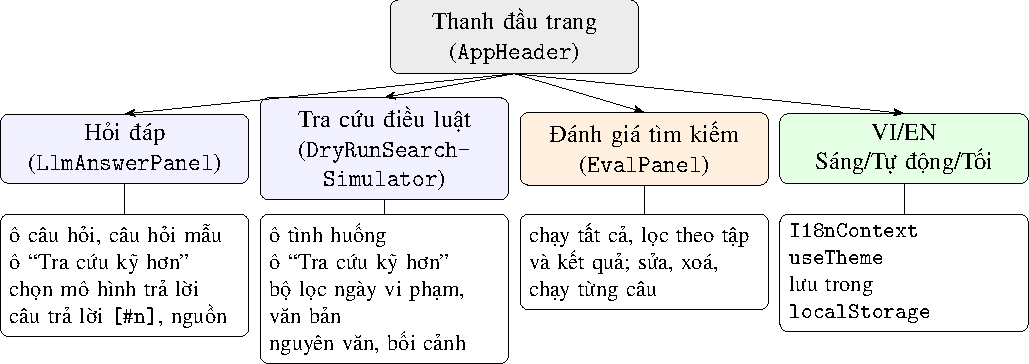
\includegraphics{graphics/fig_ch3_7.pdf}}
\caption{Cấu trúc điều hướng của giao diện}
\label{fig:dieuhuong}
\end{figure}

Giao diện được thiết kế theo bốn nguyên tắc: nguồn luôn đi cùng câu trả lời, với điều khoản nguồn và ghi chú sửa đổi hiển thị ngay bên dưới; người dùng có thể hỏi như khi nhắn tin, kể cả không dấu; kết quả có độ tương đồng thấp luôn kèm cảnh báo; và giao diện hỗ trợ hai ngôn ngữ, ba chế độ màu cùng bố cục một cột trên điện thoại.

\fussy
